\documentclass[a4paper,11pt,twoside]{report}


% -------------- Kodowanie znaków, język polski -------------

\usepackage[utf8]{inputenc}
\usepackage[MeX]{polski}
%\usepackage[T1]{fontenc}
\usepackage[english, polish]{babel}


% ----------------- Przydatne pakiety ----------------------
\usepackage{amsfonts}
\usepackage{mathrsfs} 
\usepackage{amsmath,amsthm,latexsym,xpatch}
\usepackage[dvips]{graphicx,color}
\usepackage{enumerate}
\usepackage{enumitem}
\usepackage{verbatim}
\usepackage{array}
\usepackage{pstricks}
\usepackage{textcomp}
\usepackage{listings}
\usepackage{xcolor}
\usepackage[none]{hyphenat}

% ---------------- Marginesy, akapity, interlinia ------------------

\usepackage[inner=20mm, outer=20mm, bindingoffset=10mm, top=25mm, bottom=25mm]{geometry}


\linespread{1.5}
%\allowdisplaybreaks
\usepackage{indentfirst} % opcjonalnie; pierwszy akapit z wcięciem
\setlength{\parindent}{5mm}

\hyphenation{Syl-ves-tra}
\hyphenation{Syl-ves-ter-a}

%--------------------------- ŻYWA PAGINA ------------------------

\usepackage{fancyhdr}
\pagestyle{fancy}
\fancyhf{}
% numery stron: lewa do lewego, prawa do prawego 
\fancyfoot[LE,RO]{\thepage} 
% prawa pagina: zawartość \rightmark do lewego, wewnętrznego (marginesu) 
\fancyhead[LO]{\sc \nouppercase{\rightmark}}
% lewa pagina: zawartość \leftmark do prawego, wewnętrznego (marginesu) 
\fancyhead[RE]{\sc \leftmark}

\renewcommand{\chaptermark}[1]{
\markboth{\thechapter.\ #1}{}}

% kreski oddzielające paginy (górną i dolną):
\renewcommand{\headrulewidth}{0 pt} % 0 - nie ma, 0.5 - jest linia


\fancypagestyle{plain}{% to definiuje wygląd pierwszej strony nowego rozdziału - obecnie tylko numeracja
  \fancyhf{}%
  \fancyfoot[LE,RO]{\thepage}%
  
  \renewcommand{\headrulewidth}{0pt}% Line at the header invisible
  \renewcommand{\footrulewidth}{0.0pt}
}



% ---------------- Nagłówki rozdziałów ---------------------

\usepackage{titlesec}
\titleformat{\chapter}%[display]
  {\normalfont\Large \bfseries}
  {\thechapter.}{1ex}{\Large}

\titleformat{\section}
  {\normalfont\large\bfseries}
  {\thesection.}{1ex}{}
\titlespacing{\section}{0pt}{30pt}{20pt} 
%\titlespacing{\co}{akapit}{ile przed}{ile po} 
    
\titleformat{\subsection}
  {\normalfont \bfseries}
  {\thesubsection.}{1ex}{}


% ----------------------- Spis treści ---------------------------
\def\cleardoublepage{\clearpage\if@twoside
\ifodd\c@page\else\hbox{}\thispagestyle{empty}\newpage
\if@twocolumn\hbox{}\newpage\fi\fi\fi}


% kropki dla chapterów
\usepackage{etoolbox}
\makeatletter
\patchcmd{\l@chapter}
  {\hfil}
  {\leaders\hbox{\normalfont$\m@th\mkern \@dotsep mu\hbox{.}\mkern \@dotsep mu$}\hfill}
  {}{}
\makeatother

\usepackage{titletoc}
\makeatletter
\titlecontents{chapter}% <section-type>
  [0pt]% <left>
  {}% <above-code>
  {\bfseries \thecontentslabel.\quad}% <numbered-entry-format>
  {\bfseries}% <numberless-entry-format>
  {\bfseries\leaders\hbox{\normalfont$\m@th\mkern \@dotsep mu\hbox{.}\mkern \@dotsep mu$}\hfill\contentspage}% <filler-page-format>

\titlecontents{section}
  [1em]
  {}
  {\thecontentslabel.\quad}
  {}
  {\leaders\hbox{\normalfont$\m@th\mkern \@dotsep mu\hbox{.}\mkern \@dotsep mu$}\hfill\contentspage}

\titlecontents{subsection}
  [2em]
  {}
  {\thecontentslabel.\quad}
  {}
  {\leaders\hbox{\normalfont$\m@th\mkern \@dotsep mu\hbox{.}\mkern \@dotsep mu$}\hfill\contentspage}
\makeatother



% ---------------------- Spisy tabel i obrazków ----------------------

\renewcommand*{\thetable}{\arabic{chapter}.\arabic{table}}
\renewcommand*{\thefigure}{\arabic{chapter}.\arabic{figure}}
%\let\c@table\c@figure % jeśli włączone, numeruje tabele i obrazki razem


% --------------------- Definicje, twierdzenia etc. ---------------


\makeatletter
\newtheoremstyle{definition}%    % Name
{3ex}%                          % Space above
{3ex}%                          % Space below
{\upshape}%                      % Body font
{}%                              % Indent amount
{\bfseries}%                     % Theorem head font
{.}%                             % Punctuation after theorem head
{.5em}%                            % Space after theorem head, ' ', or \newline
{\thmname{#1}\thmnumber{ #2}\thmnote{ (#3)}}%  % Theorem head spec (can be left empty, meaning `normal')
\makeatother

% ----------------------------- POLSKI --------------------------------
\theoremstyle{definition}
\newtheorem{theorem}{Twierdzenie}[chapter]
\newtheorem{lemma}[theorem]{Lemat}
\newtheorem{example}[theorem]{Przykład}
\newtheorem{proposition}[theorem]{Stwierdzenie}
\newtheorem{corollary}[theorem]{Wniosek}
\newtheorem{definition}[theorem]{Definicja}
\newtheorem{remark}[theorem]{Uwaga}

% If in English, comment this and uncomment below:

% ----------------------------- ENGLISH -----------------------------
%\theoremstyle{definition}
%\newtheorem{theorem}{Theorem}[chapter]
%\newtheorem{lemma}[theorem]{Lemma}
%\newtheorem{example}[theorem]{Example}
%\newtheorem{proposition}[theorem]{Proposition}
%\newtheorem{corollary}[theorem]{Corollary}
%\newtheorem{definition}[theorem]{Definition}
%\newtheorem{remark}[theorem]{Remark}



% ----------------------------- Dowód -----------------------------

\makeatletter
\renewenvironment{proof}[1][\proofname]
{\par
  \vspace{-12pt}% remove the space after the theorem
  \pushQED{\qed}%
  \normalfont
  \topsep0pt \partopsep0pt % no space before
  \trivlist
  \item[\hskip\labelsep
        \sc
    #1\@addpunct{:}]\ignorespaces
}
{%
  \popQED\endtrivlist\@endpefalse
  \addvspace{20pt} % some space after
}

\renewcommand{\qedhere}{\hfill \qedsymbol}
\makeatother





% -------------------------- POCZĄTEK --------------------------


% --------------------- Ustawienia użytkownika ------------------

\newcommand{\tytul}{Gogle AR jako modyfikacja gogli VR}
\renewcommand{\title}{AR googles as modified VR googles}
\renewcommand{\author}{Dawid Łazuk, Piotr Piwowarski}
\newcommand{\album}{268791,000000}
\newcommand{\type}{inżyniers} % magisters, licencjac (Master or Engineer in English)
\newcommand{\supervisor}{dr inż. Krzysztof Kaczmarski}

\lstdefinestyle{sharpc}{language=[Sharp]C, rulecolor=\color{blue!80!black}}

\begin{document}
\sloppy

% \selectlanguage{english} % uncomment this for English 

% ----------------------- Abstrakty -----------------------------

%\selectlanguage{polish}
\begin{abstract}

\begin{center}
\tytul
\end{center}

Streszczam.

Lorem ipsum dolor sit amet, consetetur sadipscing elitr, sed diam nonumyeirmod tempor invidunt ut labore et dolore magna aliquyam erat, sed diamvoluptua. At vero eos et accusam et justo duo dolores et ea rebum. Stet clita kasd gubergren, no sea takimata sanctus est Lorem ipsum dolor sit amet.\\

\noindent \textbf{Słowa kluczowe:} slowo1, slowo2, ...
\end{abstract}

\null\thispagestyle{empty}\newpage

{\selectlanguage{english}
\begin{abstract}

\begin{center}
\title
\end{center}

Lorem ipsum dolor sit amet, consetetur sadipscing elitr, sed diam nonumyeirmod tempor invidunt ut labore et dolore magna aliquyam erat, sed diamvoluptua. At vero eos et accusam et justo duo dolores et ea rebum. Stet clita kasd gubergren, no sea takimata sanctus est Lorem ipsum dolor sit amet.

Lorem ipsum dolor sit amet, consetetur sadipscing elitr, sed diam nonumyeirmod tempor invidunt ut labore et dolore magna aliquyam erat, sed diamvoluptua. At vero eos et accusam et justo duo dolores et ea rebum. Stet clita kasd gubergren, no sea takimata sanctus est Lorem ipsum dolor sit amet.\\

\noindent \textbf{Keywords:} keyword1, keyword2, ...
\end{abstract}}


\null\thispagestyle{empty}\newpage

\null \hfill Warszawa, dnia ..................\\

\par\vspace{5cm}

\begin{center}
Oświadczenie % Declaration - for English
\end{center}

\indent Oświadczam, że pracę \type ką pod
tytułem ,,\tytul '', której promotorem jest \supervisor \ wykonałam/em
samodzielnie, co poświadczam własnoręcznym podpisem.
\vspace{2cm}

% English:

%I hereby declare that the thesis entitled ,,\title '', submitted for the \type ~degree, supervised  by \supervisor , is entirely my original work apart from the recognized reference.
%\vspace{2cm}

\begin{flushright}
  \begin{minipage}{50mm}
    \begin{center}
      ..............................................

    \end{center}
  \end{minipage}
\end{flushright}

\thispagestyle{empty}
\newpage

\null\thispagestyle{empty}\newpage
% ------------------- 4. Spis treści ---------------------
% \selectlanguage{english} - for English

\tableofcontents
\thispagestyle{empty}
\newpage
% -------------- 5. ZASADNICZA CZĘŚĆ PRACY --------------------
\null\thispagestyle{empty}\newpage
\setcounter{page}{11}
\pagestyle{fancy}


\chapter*{Wstęp} % Intruduction
\markboth{}{Wstęp}
\addcontentsline{toc}{chapter}{Wstęp}

Szybki rozwój techniki spowodował zwiększenie jej obecności w codziennym życiu. Rozwój interfejsów użytkownika i badania nad jego wrażeniami z wykorzystywania różnych systemów spowodowały powstanie technologii takich jak wirtualna rzeczywistość i rozszerzona rzeczywistość. Służą one zarówno do rozrywki jak i też do ułatwienia życia i usprawnienia pracy ludziom. Rozwiązania tego typu stają się coraz popularniejsze i można zaobserwować rosnące nimi zainteresowanie w wielu branżach.

Dlatego też, w niniejszej pracy podjęto się zbadania możliwości zastosowania gogli wirtualnej rzeczywistości w aplikacjach wykorzystujących rzeczywistość rozszerzoną. Stworzony zostanie system, który umożliwia przekazanie obrazu widzianego przez kamery, symulujące ludzkie oczy, do gogli wirtualnej rzeczywistości. Powstałe w ten sposób ``wirtualne okulary'' będą mogły zostać wykorzystane do uruchomienia na nich aplikacji przeznaczonych na systemy rozszerzonej rzeczywistości.
Drugim celem pracy, po stworzeniu takiego systemu, było zbadanie czy i jak bardzo wizja uzyskana przez gogle wirtualnej rzeczywistości w połączeniu z kamerami różni się od naturalnej wizji człowieka. Czy osiągnięty efekt będzie akceptowalny dla użytkownika.

\chapter{Technologia VR/AR. Wizja ludzka.}

W tym rozdziale omówione zostaną zagadnienia wirtualnej oraz rozszerzonej rzeczywistości. Poruszone zostaną problemy, jakie wiążą się z zastosowaniem tych technologii. Przedstawiona zostanie też natura wizji stereoskopowej człowieka w zakresie zjawisk, które będą miały wpływ na przebieg prac i ich rezultat.

\section{Wirtualna i rozszerzona rzeczywistość}

\subsection{Definicje i zastosowanie VR/AR}

\begin{definition}[Wirtualna rzeczywistość]
\textit{Wirtualną rzeczywistością} (ang. VR - Virtual Reality) nazywamy wrażenie przebywania użytkownika w świecie stworzonym wirtualnie. Zwykle dotyczy to obrazu, dźwięku oraz interakcji z otoczeniem, ale podejmowane są próby wykorzystania zapachu i dotyku w aplikacjach VR.
\end{definition}

Obecnie większości ludziom termin VR kojarzy się z goglami zakładanymi na głowę użytkownika, które umożliwiają wyświetlanie sceny 3D w taki sposób, że użytkownik ma wrażenie przebywania w tej scenie. Wbudowane w urządzenie żyroskopy reagują na ruchy głowy odwzorowując je w wyświetlanym obrazie. Gogle często posiadają wbudowane głośniki (Oculus Rift) lub możliwość podpięcia słuchawek (HTC Vive), zapewniając także bodźce akustyczne. Takie rozwiązanie pozwala osiągnąć immersję nieosiągalną dla dotychczasowo wykorzystywanych technologii, nawet takich jak telewizja trójwymiarowa.

Wirtualna rzeczywistość jest obecnie stosowana na bardzo szeroką skalę. Wykorzystywana jest w przemyśle rozrywkowym w postaci gier VR czy też filmów 360\textdegree, w których użytkownik może poczuć się jakby znajdował się w samym centrum akcji. Rozwiązania VR mają potencjał w przemyśle turystycznym, umożliwiając wirtualne wycieczki po egzotycznych, często trudno dostępnych miejscach. Agenci nieruchomości mogą umożliwić zainteresowanym klientom obejrzenie mieszkania czy domu jeszcze przed powstaniem budynku. Wystarczy tylko stworzyć odpowiedni model 3D i wyświetlić go w goglach wirtualnej rzeczywistości. Technologia znalazła też zastosowanie w szkoleniu żołnierzy, umożliwiając przeprowadzenie symulacji operacji na~wirtualnych poligonach.

\textbf {źródło: http://www.komputerswiat.pl/centrum-wiedzy-konsumenta/gaming/wszystko-o-wirtualnej-rzeczywistosci/co-to-jest-wirtualna-rzeczywistosc.aspx }

\begin{definition}[Rozszerzona rzeczywistość]
\textit{Rozszerzoną rzeczywistością} (ang. AR - Augmented Reality) nazywamy nałożenie na wizję świata rzeczywistego obrazu stworzonego wirtualnie. Użytkownik dzięki temu może na przykład otrzymywać dodatkowe informacje o obiektach, na które patrzy. Systemy AR nie zapewniają interakcji z częścią wirtualną świata.
\end{definition}

Rozwiązania rozszerzonej rzeczywistości wzbogacają zmysły człowieka poprzez przekazanie im dodatkowych informacji. O ile w przypadku wirtualnej rzeczywistości użytkownik, w pewnym sensie, odcinał się od świata rzeczywistego, tak w przypadku rzeczywistości rozszerzonej ten kontakt z rzeczywistością pozostaje. Istnieją samochody oraz myśliwce wyposażone w HUD - przezroczysty ekran wyświetlający informacje takie jak na przykład prędkość, z jaką porusza się samochód, nie zasłaniając tego co za nim się znajduje. Dość znanym zastosowaniem rozszerzonej rzeczywistości jest, wydana w 2016 roku, gra Pokemon GO. Użytkownik przy pomocy swojego smartphone'a spacerując po mieście zbiera pokemony, które wyświetlają się na ekranie telefonu jako obraz nałożony na  świat rzeczywisty, widziany przez kamerę urządzenia.

Przykładami urządzeń AR obecnymi na rynku są Google Glass i Microsoft HoloLens. W odróźnieniu od wirtualnej rzeczywistości, oczy użytkownika nie zostają zasłonięte całkowicie. Urządzenia mają formę okularów, przez które człowiek widzi to co przed nim się znajduje, a obraz wirtualny jest wyświetlany na okularach bądź aplikowany bezpośrednio do oka.

\begin{definition}[Mieszana rzeczywistość]
\textit{Mieszaną rzeczywistością} (ang. MR - Mixed Reality) nazywamy rozszerzenie klasy rozwiązań AR o interakcję użytkownika z wirtualną częścią świata.
\end{definition}

Zagadnienie mieszanej rzeczywistości leży poza zakresem niniejszej pracy. Definicja została zamieszczona w celu rozróżnienia tej klasy rozwiązań od rozwiązań rozszerzonej rzeczywistości.

\subsection{ Problemy użytkowe VR/AR }

Wykorzystanie rozwiązań wirtualnej i rozszerzonej rzeczywistości niesie za sobą szereg wyzwań stawianych deweloperom, oraz konsekwencji, których użytkownicy muszą być świadomi.

\pagebreak
\begin{description}
\item [Wymogi wydajnościowe] \hfill \\
W celu komfortowego korzystania z rozwiązań wirtualnej rzeczywistości systemy muszą spełniać szereg wymogów wydajnościowych. Organizm ludzki najlepiej akceptuje obraz o częstotliwości zgodnej z częstotliwością pracy oka. Podanie obrazu o częstotliwości dużo niższej będzie powodowało dyskomfort w korzystaniu z aplikacji. Przyjmuje się, że obraz w aplikacjach VR powinien mieć $90 FPS$, a opóźnienie obrazu nie powinno przekraczać $20 ms$.
\item [Wpływ na wzrok] \hfill \\
Nie podlega wątpliwościom, że długotrwała praca przy monitorze szkodzi. Mięśnie gałki ocznej, które w normalnych warunkach są odpowiedzialne za akomodację oka, zastygają w jednej pozycji, ponieważ ekran jest w mniej więcej stałej odległości od oka. Intensywne światło też ma negatywny wpływ na oczy. W przypadku gogli wirtualnej rzeczywistości mamy do czynienia z relatywnie dużym ekranem, zasłaniającym praktycznie całe pole widzenia użytkownika, w odległości rzędu kilkudziesięciu milimetrów od oka. Długotrwała praca oczu w takich warunkach może doprowadzić do pogorszenia wzroku.
\item [Choroba symulacyjna] \hfill \\
Ludzki organizm jest skonstruowany tak, że mózg pobiera informacje dotyczące otoczenia z różnych zmysłów. W normalnych warunkach bodźce z różnych układów odbierane w tym samym czasie odpowiadają sobie. W zagadnieniach wirtualnej rzeczywistości układem zmysłów, powodującym problemy, jest układ oczy - błędnik. W grach lub filmach, w których występuje ruch, oczy użytkownika odbierają bodźce wskazujące na ruch organizmu. Natomiast jeśli użytkownik siedzi na przykład w fotelu, jego błędnik nie wykrywa ruchu. Mózg otrzymuje sprzeczne bodźce co skutkuje objawami podobnymi do choroby lokomocyjnej.
\item [Zbyt wysoka immersja] \hfill \\
Znane są przypadki ludzi umierających przed ekranem monitora po kilkunastu lub kilkudziesięciu godzinach nieustannej gry. Osoby uzależnione w takim stopniu od wirtualnej rozgrywki mają problem z rozróżnianiem świata rzeczywistego od wirtualnego, zapominając nawet o potrzebach fizjologicznych. Wysoka immersja, osiągana przez rozwiązania wirtualnej rzeczywistości, może spotęgować ten problem. Zwłaszcza, że rozrywka VR jest znacznie bardziej wymagająca dla organizmu od tradycyjnej, co już zostało wcześniej opisane. 
Kolejny problem dotyczący immersji jest związany z osobami mającymi problemy kardiologiczne. Realistyczne wrażenia z gier typu horror mogą doprowadzić takie osoby nawet do zawału serca.
\end{description}

\textbf {źródło: http://www.komputerswiat.pl/centrum-wiedzy-konsumenta/gaming/wszystko-o-wirtualnej-rzeczywistosci/niebezpieczenstwa-i-wady-vr.aspx }

\section{Wizja stereoskopowa człowieka}

Człowiek doświadcza widzenia trójwymiarowego dzięki temu, że dwoje jego oczu jest skierowane mniej więcej równolegle w ten sam punkt. Umożliwia to zebranie dwóch podobnych do siebie obrazów. Różnica między nimi polega na przesunięciu oczu (kamer) względem siebie, przez co każdy obiekt jest widziany na jednym obrazie z nieco innej perspektywy, niż na drugim. Mózg nakładając na siebie te obrazy, dzięki tej różnicy, tworzy efekt głębi umożliwiając człowiekowi ocenę odległości przedmiotów, na które patrzy.

\subsection{Odległość między źrenicami}

Badania antropometryczne personelu armii Stanów Zjednoczonych w 2012 roku objęły swoim zakresem odległości między ludzkimi źrenicami. Wyniki tych badań są zawarte w poniższej tabeli. Dane są przedstawione w milimetrach.

\begin{table}[h!]
\centering
\label{my-label}
\begin{tabular}{lcccc}
\textbf{Płeć} & \multicolumn{1}{l}{\textbf{Minimum}} & \multicolumn{1}{l}{\textbf{Maksimum}} & \multicolumn{1}{l}{\textbf{Średnia}} & \multicolumn{1}{l}{\textbf{Mediana}} \\
Kobieta       & 51.0                                 & 74.5                                  & 61.7                                 & 62.0                                 \\
Mężczyzna     & 53.0                                 & 77.0                                  & 64.0                                 & 64.0                                
\end{tabular}
\caption{Odległości między źrenicami}
\end{table}

Z powyższych danych jednoznacznie wynika, że odległość pomiędzy ludzkimi źrenicami zawiera się w przedziale od 51.0 milimetrów do 77.0 milimetrów.

\textbf{(http://www.dtic.mil/docs/citations/ADA634277 - do przypisów)}

\subsection{Akomodacja oka}

\begin{definition}[Akomodacja oka]
\textit{Akomodacją oka} nazywamy zjawisko dostosowania się soczewki oka do odległości od oglądanego przedmiotu, w celu zapewnienia ostrości obrazu.
\end{definition}

U człowieka akomodacja oka jest realizowana poprzez zmianę kształtu soczewki, co skutkuje zmianą jej ogniskowej (zdolności skupiającej).

\begin{definition}[Punkt bliży wzrokowej]
\textit{Punktem bliży wzrokowej} nazywamy minimalną odległość, przy której akomodacja oka wpływa na ostrość obrazu. U człowieka punkt bliży wzrokowej leży w odległości $10 cm$ od oka.
\end{definition}

\begin{minipage}{\linewidth}
\begin{definition}[Punkt dali wzrokowej]
\textit{Punktem dali wzrokowej} nazywamy maksymalną odległość, przy której akomodacja oka wpływa na ostrość obrazu. U człowieka punkt dali wzrokowej leży w odległości $6 m$ od oka.
\end{definition}
\end{minipage}

\subsection{Zbieżność oczu}

\begin{definition}[Zbieżność oczu]
\textit{Zbieżnością oczu} nazywamy zjawisko obrócenia oczu do środka w sytuacji, kiedy obserwowany punkt leży w niewielkiej odległości od obserwatora. W takim przypadku osie widzenia obu oczu przecinają się w jednym punkcie. Jeżeli natomiast obserwowany punkt leży daleko od obserwatora, osie widzenia są równoległe do siebie.
\end{definition}

\begin{figure}[h]
\centering
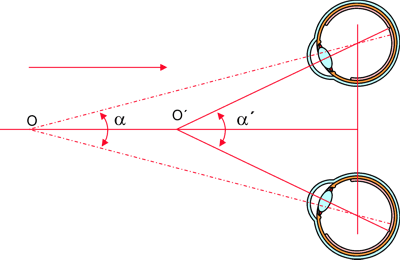
\includegraphics[scale=0.5]{zbieznosc}
\caption[Zbieżność oczu (źródło: http://www.swiatlo.tak.pl/1/index.php/funkcje-wzroku-akomodacja-adaptacja-zbieznosc/)]{Zbieżność oczu}
\end{figure}

\chapter{Cel i założenia projektu} % Cel i założenia projektu

Rozdział poświęcony jest opisaniu celu projektu, który powstaje w ramach niniejszej pracy inżynierskiej. Wyspecyfikowane zostaną wymagania, jakie tworzony system musi spełniać.

\section{Funkcjonalność systemu}

System ma umożliwiać przekazanie obrazu z dwóch kamer do gogli wirtualnej rzeczywistości, tworząc tym samym gogle rozszerzonej rzeczywistości. Takie gogle następnie będą mogły posłużyć do wykorzystywania aplikacji przeznaczonych na rozwiązania AR. 

System ma umożliwiać efekt widzenia stereoskopowego, aby użytkownik miał wrażenie wizji zbliżonej do naturalnej, trójwymiarowej wizji człowieka. Efekt ten zostanie osiągnięty poprzez umiejscowienie kamer tak, aby odległość między ich soczewkami odpowiadała odległości pomiędzy źrenicami ludzkich oczu. 

System ma umożliwiać przetwarzanie przechwyconego obrazu zanim trafi on do oczu. Przetwarzanie to może być realizowane na przykład poprzez nałożenie prostych filtrów na obraz, lub też wykorzystania bardziej zaawansowanych algorytmów (na przykład wykrywania twarzy).

\section{Środowisko sprzętowe}

W tym podrozdziale omówione zostaną urządzenia wykorzystane w pracy. Przedstawiona zostanie specyfikacja sprzętu zapewnionego przez Wydział Matematyki i Nauk Informacyjnych Politechniki Warszawskiej. Omówimy także problemy wynikające z wykorzystania danego rodzaju sprzętu oraz propozycje ich rozwiązania.

\subsection{Gogle Oculus Rift}

Oculus Rift to gogle wirtualnej rzeczywistości stworzone przez firmę Oculus VR, będącą obecnie własnością Facebook Inc. Zostały ujawnione światu w 2012 roku na platformie Kickstarter w celu zebrania funduszy na rozwój projektu. 

Oculus Rift wykorzystuje dwa ekrany OLED, po jednym na każde oko. Ekrany te mają rozdzielczość 1080 pikseli na 1200 pikseli. Częstotliwość ich odświeżania wynosi 90 Hz. Pomiędzy ekranami, a oczami użytkownika znajdują się soczewki. Kąty widzenia gogli to 90\textdegree  pionowo i 80\textdegree  poziomo.

Gogle zostaną wykorzystane do wyświetlania obrazu przechwyconego przez kamery.

\subsection{Logitech Webcam C910 Pro HD}

C910 Pro HD to kamera USB stworzona przez firmę Logitech. Umożliwia przechwytywanie obrazu o rozdzielczości 1920 pikseli na 1080 pikseli. Posiada wbudowany mikrofon, jednak nie będzie on wykorzystywany w naszej pracy.

Wydział MiNI zapewnił dwa egzemplarze tych kamer na rzecz niniejszej pracy. W związku z tym, że panoramiczny obraz, standardowo zapewniany przez kamery, jest daleki od natury ludzkiego oka ograniczymy się do obrazu 4:3. Zatem rozdzielczość obrazu w naszej pracy będzie wynosiła 1440 pikseli na 1080 pikseli na jedno oko.

Obudowa tej kamery jest dość duża, szczególnie w pozycji poziomej. Jest to problematyczne, ponieważ minimalna odległość między soczewkami, na jaką możemy umieścić kamery w tej pozycji, wynosi około 100 milimetrów. Jest to znacznie powyżej górnego ograniczenia odległości między ludzkimi źrenicami. W związku z tym konieczne będzie umieszczenie tych kamer w pozycji pionowej. Skutkuje to tym, że efektywna rozdzielczość przechwytywanego obrazu będzie wynosiła 1080 pikseli na 1440 pikseli.

\section{Odwzorowanie wizji stereoskopowej}

Uzyskanie efektu wizji trójwymiarowej podczas używania gogli z zaimplementowanym rozwiązaniem jest jednym z najważniejszych celów tego projektu. W tym podrozdziale znajduje się odniesienie do cech wizji stereoskopowej, opisanych w poprzednim rozdziale, pod kątem tego, jak wpływają na tworzone rozwiązanie w ramach niniejszej pracy. 

\pagebreak
\subsection{Parametryzacja wizji}

Wizję stereoskopową można opisać trzema parametrami:

\begin{itemize}
\item Kąt widzenia kamer
\item Odległość między obiektywami kamer
\item Kąt odchylenia osi widzenia
\end{itemize}

Pierwszy z tych parametrów - kąt widzenia kamer, jest zależny bezpośrednio od modelu kamery zastosowanego w projekcie. Jedyna możliwa jego regulacja polega na obcięciu brzegów obrazu, zmniejszając tym samym kąt widzenia. W niniejszej pracy istotnym jest, aby kąt widzenia kamer był zbliżony do kąta widzenia zapewnianego przez gogle Oculus Rift.

Dwa kolejne - odległość między kamerami i odchylenie osi widzenia, są istotne przy uzyskaniu efektu głębi podczas patrzenia przez gogle. Przy założeniu, że obserwujemy jeden punkt, istnieje korelacja między tymi parametrami pozwalająca uzyskać efekt głębi patrząc na przedmioty w okolicy obserwowanego punktu nawet w syttuacji, gdy odległość, bądź odchylenie odbiegają od idealnego ustawienia dla danego użytkownika. Przykładem będzie odchylenie osi widzenia do środka w przypadku, gdy odległości między obiektywami są większe, niż między oczami użytkownika. Jednakże efekt w ten sposób uzyskany jest tylko punktowy, a obiekty położone w innej odległości od punktu odniesienia nie będą widziane jako trójwymiarowe.

\subsection{Cechy ludzkiej wizji w projekcie}

W podrozdziale \textit{Wizja stereoskopowa człowieka} zostały przedstawione cechy ludzkiej wizji, które mają wpływ na przebieg niniejszej pracy. W tym podrozdziale omówione zostaną założenia, jakie zostały podjęte podczas realizacji projektu w celu spełnienia tych wymagań, oraz uzasadnienie w przypadku braku możliwości spełnienia danego wymagania.

\begin{description}

\item[Odległość między źrenicami] \hfill \\
W celu zapewnienia komfortowego korzystania z systemu jak największej grupie użytkowników konieczne jest opracowanie sposobu umieszczenia kamer zapewniającego:
\begin{itemize}
\item Umieszczenie kamer w stałej odległości od siebie podczas użytkowania systemu
\item Regulację odległości kamer od siebie
\end{itemize}

Kamery docelowo miały zostać umieszczone na goglach, ale przewidziana jest możliwość mocowania ich na czym innym, jednak z zachowaniem punktów wymienionych powyżej.

\item [Akomodacja oka] \hfill \\
Zjawisko akomodacji oka w niniejszej pracy jest nie do odwzorowania z wykorzystaniem dostępnego sprzętu. Wymaga ono śledzenia gałki ocznej w celu wyznaczenia punktu, który jest obserwowany przez użytkownika, a następnie wyostrzenie obrazu w danym punkcie. Gogle Oculus Rift nie mają obecnie takiej możliwości.

\item[Zbieżność oczu] \hfill \\
Zjawisko zbieżności oczu w niniejszej pracy również jest nie do odzworowania z takich samych powodów co zjawisko \textit{akomodacji oka}. Należałoby wyznaczyć punkt obserwowany przez użytkownika, a następnie skierować kamery w dany punkt. Wymagałoby to też stworzenia urządzenia, które poruszałoby kamerami w zależności od obserwowanego punktu. Wykracza to znacznie poza zakres tej pracy.

\end{description}

\chapter{Implementacja projektu}

W tym rozdziale przedstawione zostaną efekty pracy. Omówione zostaną decyzje architektoniczne oraz szczegóły techniczne zaimplementowanego rozwiązania.

\section{Wybrane technologie i oprogramowanie}

\subsection{Języki i technologie }

\begin{description}
\item [Język programowania C\# ] \hfill \\
System został wykonany z wykorzystaniem języka programowania C\# oraz platformy programistycznej .NET Framework. Wybór tej technologii był podyktowany doświadczeniem zespołu w jej wykorzystaniu. Również wykorzystany silnik Unity3D wspiera .NET co sugerowało uniknięcie przyszlych problemów integracją modułów. W pracy .NET Framework został wykorzystany do napisania funkcjonalności pobierania obrazu z kamer i przetwarzania go, zanim trafi do modułu przekazywania obrazu do gogli.

\item [EmguCV] \hfill \\
Biblioteka opakowująca popularną bibliotekę do przetwarzania obrazów - OpenCV, w interfejs umożliwiający wykorzystanie jej w aplikacjach napisanych w języku C\#. Wykorzystana do implementacji modułów przechwytywania i przetwarzania obrazu. Przykładowe algorytmy przetwarzania obrazu również zostały napisane z wykorzystaniem tej biblioteki.

\item [Silnik Unity3D] \hfill \\
Zintegrowane środowisko do tworzenia trójwymiarowych gier i innych materiałów interaktywnych.  Pozwala tworzyć aplikacje na przeglądarki internetowe, komputery osobiste, konsole gier wideo oraz urządzenia mobilne. Środowisko to zostało wybrane ze względu na łatwą integrację z pozostałymi używanymi technologiami. Zostało wykorzystane do stworzenia warstwy przekazywania obrazu do gogli OculusRift.

\begin{minipage}{\linewidth}
\item [Windows Presentation Foundation] \hfill \\
Windows Presentation Foundation (WPF) jest technologią służącą do tworzenia interfejsów użytkownika w aplikacjach desktopowych w środowisku .NET. W niniejszej pracy technologia ta została wykorzystana do napisania aplikacji konfiguracyjnej, która szerzej opisana będzie w dalszej części pracy.
\end{minipage}\\

\item [Windows Communication Foundation] \hfill \\
Windows Communication Foundation (WCF) jest technologią integrującą i unifikującą wszystkie technologie służące do komunikacji międzyprocesowej w aplikacjach opartych o .NET Framework. W niniejszej pracy WCF został wykorzystany do zaimplementowania komunikacji pomiędzy procesem głównym systemu, a aplikacją konfiguracyjną.
\end{description}

\subsection{Oprogramowanie}

\begin{description}
\item [Microsoft Visual Studio] \hfill \\
Zintegrowane środowisko programistyczne firmy Microsoft. Jest to najpopularniejsze IDE wykorzystywane w tworzeniu aplikacji opartych o .NET Framework.
\item [SoapUI] \hfill \\
Aplikacja służąca do testów serwisów webowych. Wykorzystana przez nas do testów połączenia pomiędzy procesem głównym, a aplikacją konfiguracyjną.
\end{description}

\section{Schemat systemu}

\subsection{Droga obrazu}

Planując wykonanie projektu droga, jaką musi przebyć obraz od przechwycenia go przez kamery do przekazania go do oka użytkownika, została podzielona na trzy warstwy. Są to:

\begin{description}
\item [Warstwa przechwytywania obrazu] \hfill \\ Jest odpowiedzialna za pobieranie obrazów z kamer i przygotowanie ich do dalszego przetwarzania - rotację obrazu w zależności od położenia kamery.
\item [Warstwa przetwarzania obrazu] \hfill \\ Wykonuje przetwarzanie obrazu według algorytmów zdefiniowanych przez użytkownika lub programistę.
\item [Warstwa przekazywania obrazu do gogli] \hfill \\ Odpowiada za konwersję obrazu do postaci przyjmowanej przez gogle VR.
\end{description}

\subsection{Architektura systemu}

System składa się z modułów realizujących ściśle określone zadania, dlatego też łatwo wydzielić je do osobnych projektów. Poniższy schemat przedstawia architekturę rozwiązania wraz z zaznaczonym kierunkiem przekazywania obrazu pomiędzy warstwami. 

\begin{figure}[h]
\centering
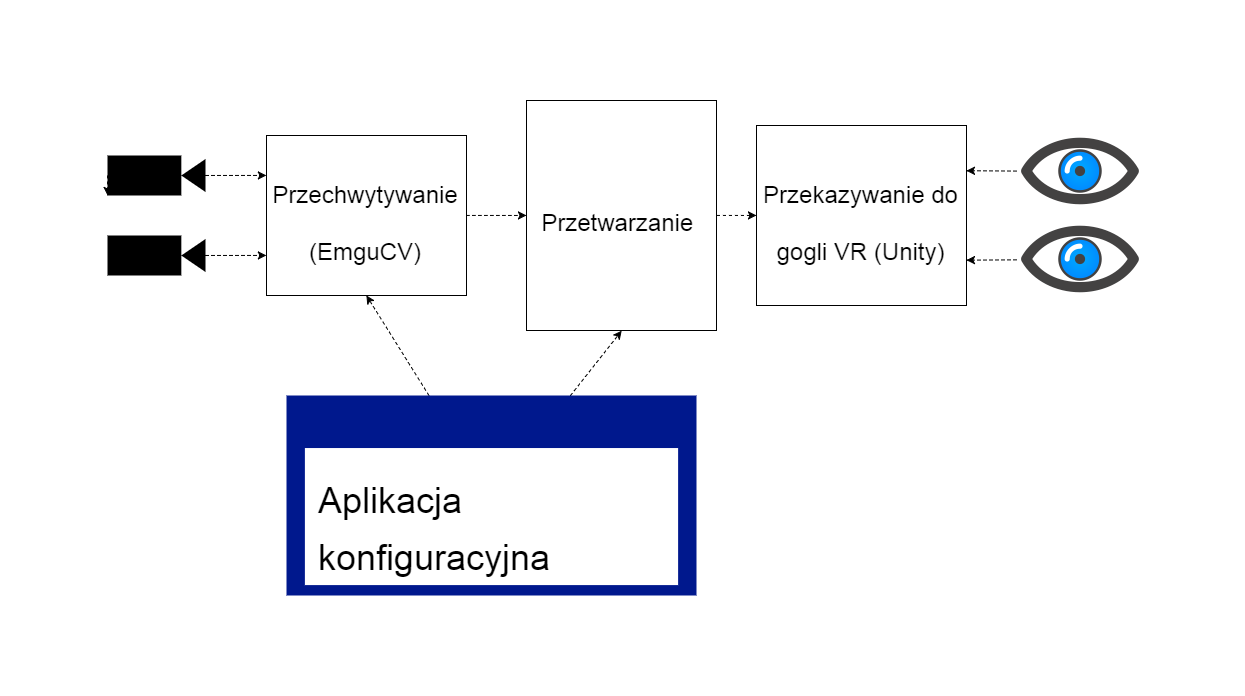
\includegraphics[scale=0.4]{architecture_schema}
\caption[Architektura systemu]{Architektura systemu}
\end{figure}

Jak widać na rysunku, obraz zanim trafi do oka przechodzi przez wszystkie warstwy. Najpierw przy użyciu biblioteki EmguCV obraz jest pobierany z kamer. Następnie przy użyciu stworzonych na potrzeby systemu klas stosowane są dla niego odpowiednie przekształcenia. Końcowy efekt osiągany jest poprzez przesłanie przetworzonego obrazu do gogli VR za pomocą aplikacji działającej przy użyciu silnika Unity. Aplikacja konfiguracyjna stworzona z wykorzystaniem technologii WPF umożliwia modyfikację parametrów w warstwach przechwytywania i przetwarzania obrazu podczas działania systemu. 

W celu zapewnienia poprawnego działania systemu, niezbędne są warstwy przechwytywania obrazu z kamer oraz przekazywania go do gogli. Warstwa przetwarzania obrazu jest opcjonalna i mogłaby być usunięta lub chwilowo wyłączona z systemu, bez utraty jego podstawowych funkcjonalności. Równolegle do pozostałych warstw (nie bierze bezpośredniego udziału w drodze obrazu od kamer do oczu) działa  aplikacja konfiguracyjna, która zapewnia graficzny interfejs do sterowania działaniem systemu. Aplikacja działa w osobnym procesie, komunikując się z głównym procesem za pomocą WCF.

\subsection{Funkcjonalność przetwarzania obrazu}

Funkcjonalność ta realizowana jest poprzez zastosowanie serii przekształceń do obrazu podczas jego drogi do oczu użytownika. System przewiduje możliwość dodawania własnych przekształceń obrazu po odpowiednim ich utworzeniu według kontraktu ustalonego w dostarczonej biltiotece programistycznej. Przekształcenia realizowane są w pewnej ustalonej kolejności. Sterowanie procesem przetwarzania obrazu realizowane jest poprzez możliwość zmiany kolejności aplikowanych przekształceń oraz wyłączenia części z nich.

\section{Opis modułów}


\subsection{Moduł przechwytywania obrazu}

W tym module zaimplementowane są wszystkie operacje powiązane z kamerami. Kontrakt tego modułu przedstawia się następująco:

\begin{figure}[h]
\centering
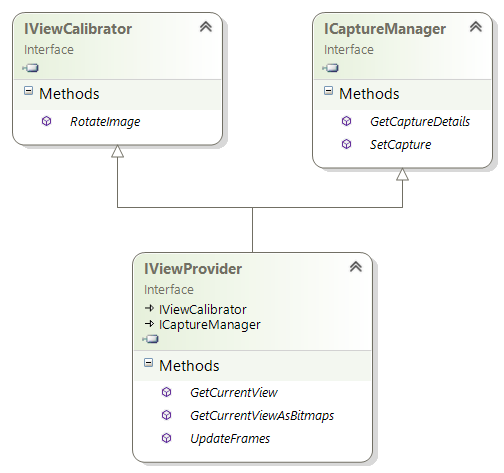
\includegraphics[scale=0.9]{IViewProvider}
\caption[Przechwytywanie diagram]{Interfejsy przechwytywania obrazów}
\end{figure}

Interfejs \textit{IViewCalibrator} jest odpowiedzialny za operacje związane z kalibracją obrazu. W tym projekcie jedyną taką operacją jest obrót obrazu w celu zrównoważenia ewentualnego obrotu kamery (metoda \textit{RotateImage}).
Interfejs \textit{ICaptureManager} odpowiada za wszystko co jest związane z przechwytywaniem obrazu. Metoda \textit{SetCapture} ustawia dany kanał na kamerę o danym indeksie w systemie, a metoda \textit{GetCaptureDetails} pobiera informacje o przechwytywanym obrazie, na przykład rozdzielczość obrazu, jego rotację czy indeks kamery, z której pochodzi.
Interfejs \textit{IViewProvider} jest głównym interfejsem, który jest implementowany przez moduł. Obejmuje sobą funkcjonalności interfejsów poprzednio wymienionych oraz udostępnia metody bezpośrednio związane z pobieraniem obrazu. Metoda \textit{UpdateFrames} wysyła sygnał do wątków pobierających obraz, aby pobrały kolejną klatkę. Pozostałe dwie metody - \textit{GetCurrentView} i \textit{GetCurrentViewAsBitmaps} pobierają obecne klatki w różnych formatach. Pierwsza z nich, wykorzystywana przez proces główny, pobiera obraz jako klasy Image biblioteki EmguCV. Druga jest wykorzystywana przez aplikację konfiguracyjną, a obraz pobrany z jej wykorzystaniem jest postaci klas System.Drawing.Bitmap.

Z powyższego opisu wynika, że najważniejsze operacje modułu to:
\begin{itemize}
\item Wybór kamery dla danego kanału.
\item Pobranie obrazu z wybranych kamer dla obu kanałów
\item Obrót obrazu w celu zrównoważenia ewentualnego obrotu kamery.
\end{itemize}

Poniżej są przedstawione zasady działania każdej z tych operacji:
\begin{description}
\item [Wybór kamery dla danego kanału] \hfill \\
Dla każdego kanału w module jest pole, w którym jest przechowywany obiekt odpowiedzialny za komunikację z daną kamerą. Do tych pól odwołują się pozostałe funkcjonalności, pobierające obraz. W przypadku zmiany kamery w danym kanale, wartość odpowiedniego pola jest podmieniana na obiekt odpowiadający kamerze docelowej. Zmiana ta jest transparentna dla pozostałych funkcjonalności.
\item [Pobranie obrazu z wybranych kamer dla obu kanałów] \hfill \\
Operacja jest zrealizowana wielowątkowo. Każdy z dwóch kanałów ma swój wątek, czeka na sygnał pobrania klatki, pobiera klatkę wykonując jednocześnie jej obrót, wysyła sygnał informujący o zakończeniu pobierania klatki. Operacje te wykonują się w pętli dopóki wątek nie zostanie przerwany.

\pagebreak
\item [Obrót obrazu w celu zrównoważenia ewentualnego obrotu kamery] \hfill \\
Moduł przechowuje informację o ilości obrotów o kąt prosty obrazu dla danego kanału. Zwiększenie (zmniejszenie) kąta obrotu polega na inkrementacji (dekrementacji) tej wartości poprzez wywołanie odpowiedniej metody. Na podstawie tej wartości przy pobraniu każdej klatki obliczany jest kąt, o który dany obraz ma być obrócony.
\end{description}

Funkcjonalności modułu są współdzielone przez aplikację główną oraz konfiguracyjną. Ta część kontraktu, która jest wykorzystywana przez aplikację konfiguracyjną, jest wydzielona jako kontrakt serwisu udostępnionego tej aplikacji, zgodnie ze wzorcem projektowym \textit{fasada}. Dzięki temu ukryte zostały zbędne funkcjonalności modułu z punktu widzenia aplikacji konfiguracyjnej upraszczając jego interfejs.

Podczas testów modułu wystąpiły sytuacje, gdzie aplikacja zawieszała się na wywołaniu metody z biblioteki EmguCV pobierającej kolejną klatkę z kamery. Występowało to w sytuacji, kiedy obiekt odpowiedzialny za pobieranie obrazu był ustawiony na kamerę, która nie istniała w systemie (jej indeksowi nie odpowiadało żadne urządzenie). Moduł zawiera rozwiązanie zapobiegające tego typu sytuacjom. Przy każdym pobraniu klatki do odpowiedniego pola jest zapisany czas jej pobrania. Podczas tworzenia instancji modułu tworzony i uruchamiany jest wątek, który co jakiś czas sprawdza czas od odstatniego pobrania klatki dla kanału. Jeżeli jest on większy od ustalonego dopuszczalnego maksimum, to wątek tego kanału jest przerywany, a w jego miejsce tworzony nowy. 
W zaimplementowanym rozwiązaniu maksymalna dopuszczalna przerwa między klatkami i czas co jaki jest ona sprawdzana wynosi 10 sekund.

\subsection{Moduł przetwarzania obrazu}

Moduł ten odpowiedzialny jest za realizację warstwy pośredniej w  systemie, czyli przetwarzania obrazów po przechwyceniu ich z kamer. Za pojedyńcze przekształcenia obrazu odpowiedzialne są klasy implementujące odpowiedni interfejs. Obiekty tych klas znajdują sie na liscie, z której są wywoływane w kolejności występowania. Programista korzystający z biblioteki może dodawać własne implementacje klas przetwarzających obraz i dodawać ich instancje do listy, co umożliwia kontrolę procesu przetwarzania obrazu odbywającego się w tej części systemu. 

Kluczowym elementem modułu jest sposób włączenia warstwy przetwarzania obrazu w proces przekazywania obrazu od kamery do gogli. Dodatkowo stworzony został kontrakt definiujący metody, które muszą posiadać klasy realizujące operacje przekształceń obrazu.

\begin{description}


\begin{minipage}{\linewidth}
\item [Funkcjonalność przetwarzania obrazu] \hfill \\
\end{minipage}

\begin{figure}[h]
\centering
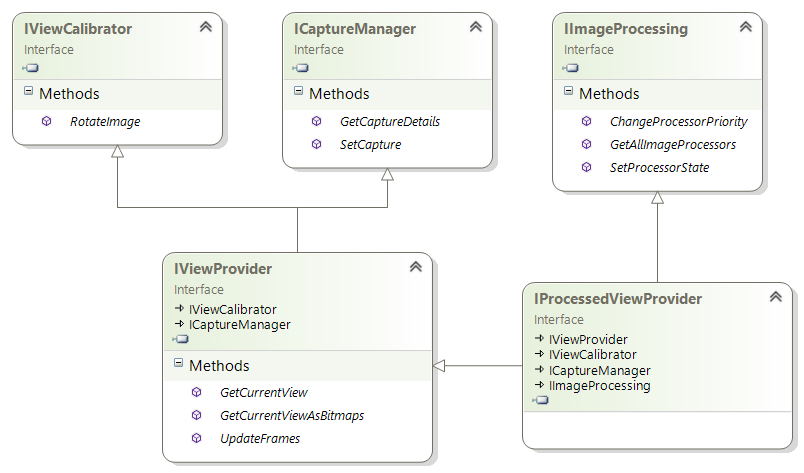
\includegraphics[scale=0.9]{IProcessedViewProvider}
\caption[Przetwarzanie diagram]{Interfejsy przetwarzania obrazów}
\end{figure}

Metoda \textit{GetAllImageProcessors} zwraca listę nazw wszytkich dostępnych obiektów przekształcających obraz wraz z informacją o ich aktywności.
Metoda \textit{SetProcessorState} pozwala zmienić stan wskazanego procesora na nieaktywny lub aktywny.
Natomiast metoda \textit{ChangeProcessorPriority} pozwala zmienić kolejność wskazanego procesora podczas procesu przetwarzania obrazu. 

Klasą bazową odpowiedzialną za pobieranie obrazu jest \textit{ViewProvider}, implementująca interfejs \textit{IViewProvider}. W celu wprowadzenia nowej warstwy aplikacji odpowiedzialnej za przetwarzanie obrazu, został stworzony interfejs \textit{IProcessedViewProvider} będący rozszerzeniem poprzedniego o dodatkowe metody związane z zarządzaniem przekształceniami obrazu, które znalazły się w interfejsie \textit{IImageProcessing}. Dodatkowo został zastosowany wzorzec projektowy \textit{Dekorator} poprzez utworzenie nowej klasy \textit{ProcessedViewProvider} implementującej interfejs \textit{IProcessedViewProvider}, będącej rozszerzeniem klasy \textit{ViewProvider} i jej interfejsu, lecz zachowującą część tych samych metod lecz o zmienionym działaniu.

Klasa ta w konstruktorze jako argument przyjmuje obiekt implementujący interfejs \textit{IViewProvider}. Kolejnym argumentem przekazywanym w konstruktorze jest lista obiektów implementujących interfejs \textit{IImageProcessor}. W metodach \textit{GetCurrentView} oraz \textit{GetCurrentViewAsBitmaps} po pobraniu obrazów z pierwotnego obiektu klasy \textit{ViewProvider} wykonywana jest seria przekształceń za pomocą obiektów znajdujących się na wspomnianej liście. W kolejności ich występowania, wywoływana jest metoda \textit{Process} której jako argument przekazywana jest referencja do obiektu reprezentującego obraz. W ten sposób obrazy zwracane w tych metodach przechodzą przez warstwę przetwarzania obrazów.

\item [Interfejs łączący implementacje przekształceń obrazu] \hfill \\

\begin{figure}[h]
\centering
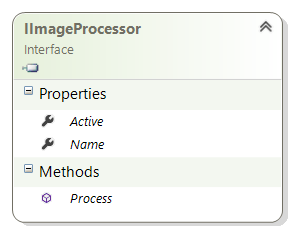
\includegraphics[scale=0.9]{IImageProcessor}
\caption[Przekształcenie diagram diagram]{Interfejs obiektu przekształcającego obraz}
\end{figure}

Metoda \textit{Process} jako argument przyjmuje referencje do obrazu reprezentowanego za pomocą typu Image<Bgr, byte> pochodzącego z biblioteki EmguCV. Operowanie na tym typie pozwala wykorzystać metody pochodzące ze wspomnianej biblioteki, co pozwalaja na szybszą konwersję obrazu przeprowadzając część operacji przy wykorzystaniu karty graficznej. Metoda nie zwraca żadnej wartosci lecz operuje na przekazanym obrazie stosując dla niego zaimplementowane przekształcenia.  \\
Dodatkowo interfejs wymaga posiadania przez klasy następujących własciwosci:
\begin{itemize}
\item  \textit{Name}, typu tekstowego - zawierająca nazwę przekształcenia.
\item \textit{Active}, typu logicznego -  decydująca o tym czy przekształcenie będzie wykonane.
\end{itemize}

\end{description}

\subsection{Moduł przekazywania obrazu do gogli}

W tym module znajdują sie wszystkie operacje związane z przekazywaniem przechwyconego obrazu z kamer do gogli. Poprzednie moduły zaimplementowano przy użyciu języka C\# oraz  platformy .NET. Dlatego do przekazywania obrazu do gogli OculusRift został wykorzystany silnik Unity3d umożliwiający importowanie zewnętrznych bibliotek stworzonych w tych technologiach.

Unity3d jest silnikiem grafiki 3D i w podstawowej wersji nie wspiera obsługi urządzeń VR. Jednak producenci gogli zapewniają dedykowane biblioteki programistyczne dla swoich urządzeń oparte na tym silniku. Pozwalają one na dodanie obsługi wirtualnej rzeczywistosci oraz sterowanie przekazywanym obrazem dla każdego oka osobno. Wykorzystany został pakiet \textit{Oculus Utitites for Unity} udostępniany przez producenta gogli OculusRift (https://developer.oculus.com/downloads/unity/), który w samym edytorze silnika Unity fukncjonuje pod nazwą \textit{OVR plugin}.  \hfill \\

\pagebreak

\begin{figure}[h]
\centering
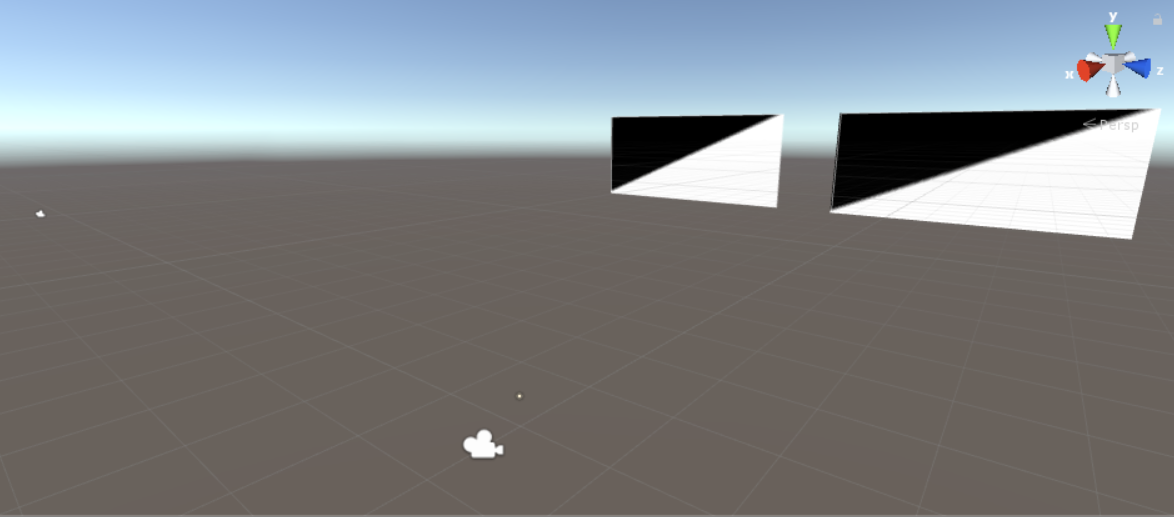
\includegraphics[scale=0.5]{unityscene}
\caption[Scena Unity]{Scena w programie Unity Editor}
\end{figure}

Wykorzystując funkcjonalnosci tego pakietu, stworzona została scena w silniku Unity zawierająca dwie kamery i dwie tekstury. Kamery posiadają właciwość o nazwie \textit{TargetEye} która pozwala decydować czy obraz w polu widzenia kamery trafia do lewego lub prawego ekranu (oka) w urządzeniu OculusRift. Na każdej z tekstur również wyświetlany jest obraz tylko dla jednego oka. Tekstury renderowane są jedynie w polu widzenia odpowiedniej kamery, zamiast być wyświetlane jak standardowy obiekt sceny. Dzięki temu podczas obrotów kamery po wykryciu ruchu urządzenia VR, tekstura nie jest poddawana żadnym przekształceniom związanym z grafiką 3D  co wpływa na wydajność systemu. W celu wyświetlenia obrazu jako tekstury potrzebna jest jego odpowiednia konwersja, która jest również ważną częścią modułu.


W module zostały przewidziane następujące interfejsy, zapewniające metody do realizacji kluczowych jego elementów.

\begin{figure}[h]
\centering
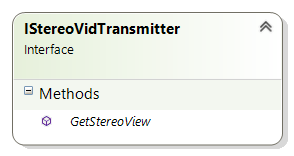
\includegraphics[scale=0.9]{IStereoVidTransmitter}
\caption[Przekazywanie diagram]{Interfejs zwracający tekstury do wyświetlenia}
\end{figure}

Interfejs \textit{IStereoVidTransmitter} jest odpowiedzialny za dostarczenie obrazów w odpowiednim formacie, gotowych do wyświetlenia na scenie programu Unity. Metoda \textit{GetStereoView} zwraca obiekt zawierający dwie tekstury - dla lewego i prawego oka. 

\begin{figure}[h]
\centering
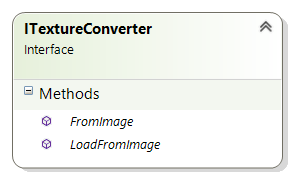
\includegraphics[scale=0.9]{ITextureConverter}
\caption[Konwersja diagram]{Interfejs dokonujący konwersji obrazu do tekstury}
\end{figure}

\begin{minipage}{\linewidth}
Interfejs \textit{ITextureConverter} odpowiada za wszystkie operacje potrzebne przy konwersji obrazu do tekstury. W systemie wykorzystywany jest przez klasy implementujące interfejs \textit{IStereoVidTransmitter}. Metoda \textit{FromBitmap} zwraca nowy obiekt tekstury utworzony na podstawie przekazanego obrazu za pomocą typu \textit{System.Drawing.Bitmap}. Metoda\textit{FromImage} działa analogicznie do poprzedniej, jednak jako argument przyjmuje obraz reprezentowany za pomocą typu z biblioteki EmguCV.
Metoda \textit{DataFromImage} zwraca tablice typu \textit{byte} z przekazanego do niej obrazu, która potrzebna jest do konwersji obrazu na teksturę w silniku Unity. Natomiast metoda \textit{LoadFromImage}  ładuje przekazany obraz do wskazanej, istniejącej tekstury. Jest wykorzystywana jest w celu poprawy wydajności i uniknięcia niepotrzebnego tworzenia tesktur przy każdej konwersji obrazu.
\end{minipage}

Z powyższego opisu wynika, że najważniejsze operacje modułu to:
\begin{itemize}
\item Przekazanie i wyświetlanie obrazu
\item Konwersja obrazu
\end{itemize}

Poniżej są przedstawione zasady działania każdej z tych operacji:

\begin{description}
\item [Przekazanie i wyświetlanie obrazu] \hfill \\
Po uruchomieniu aplikacji Unity, wraz ze stworzeniem sceny ładowany jest skrypt działający przez cały czas działania aplikacji. W skrypcie tym inicjowane  są klasy odpowiadające za pobieranie obrazu z kamer i poddanie go odpowiednim przekształceniom. Za każdym razem, gdy silnik Unity próbuje odświeżyć obraz, pobierane są dwie klatki obrazu ze wspomnianych klas - dla lewego i prawego oka. Następnie obrazy konwetowane są do postaci tekstury silnika Unity. Po ich przygotowaniu, tekstury na scenie są aktualizowane i do kamer, a później do gogli trafia odwieżony obraz.
\item [Konwersja obrazu] \hfill \\
Konwersja nie odbywa się w pełni wielowątkowo. Wszystkie peracje na obiektach silnika Unity mogą być realizowane tylko w głównym wątku (dzieje się tak ponieważ Unity automatycznie wykonuje częsć operacji na karcie graficznej i ich synchronizacja z wielu wątków jest trudna do zrealizowania). Jednak w celu maksymalnego poprawienia wydajności, w osobnych wątkach, obrazy zamieniane są na reprezentujące je tablice bajtów. Dopiero sam proces ładowania danych z tych tablic do tekstury następuje synchronicznie w głównym wątku. 
\end{description}

\subsection{Aplikacja konfiguracyjna}

Moduł ten zrealizowany został w projekcie \textit{ViewVisualization}. W jego ramach została stworzona aplikacja umożliwiająca sterowaniem obrazem trafiającym do gogli.

Do wykonania aplikacji został użyty framework \textit{WPF} (Windows Presentation Foundation). Umożliwia w wygodny sposób pogląd obrazu trafiającego do gogli oraz zmianę określonych parametrów sterujących nim. Aplikacja działa jako osobny proces, który komunikuje się z procesem aplikacji silnika Unity i może działać na innym komputerze. Komunikacja jest możliwa ponieważ w aplikacji Unity tworzony jest serwis, który umożliwia wywoływanie odpowiednich metod z klasy zajmującej się pobieraniem i przetwarzaniem obrazu (implementacja interfejsu \textit{IViewProvider}). Szczegółowy opis tego serwisu, którego kontrakt został zdefiniowany przy pomocy interfejsu \textit{IViewProviderService} znajduje się w oddzielnym, poświęconym mu rozdziale. Całość aplikacji zrealizowana jest w jednym głównym widoku \textit{MainWindow}, który pojawia się po uruchomieniu aplikacji. 

\begin{figure}[h]
\centering
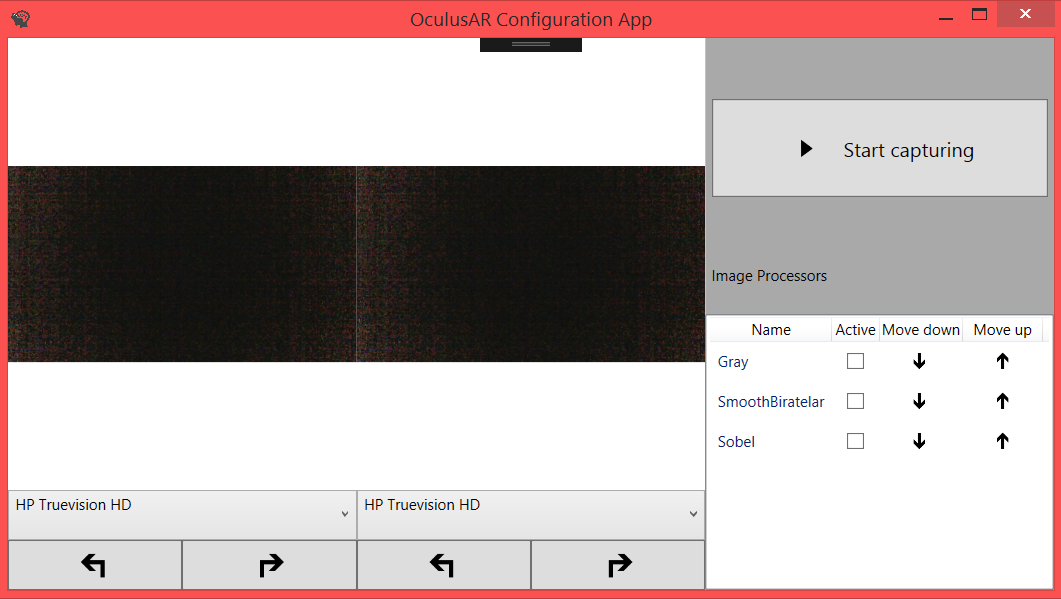
\includegraphics[scale=0.4]{mainwindow_screen}
\caption[Widok aplikacji]{Główny widok aplikacji konfiguracyjnej}
\end{figure}

Widok ten można podzielić na dwie części ze względu na spełniane funkcjonalności. 

\begin{itemize}
\item Wybór źródła i rotacji obrazu
\item Kontrola przetwarzania obrazu
\end{itemize}

W celu większej przejrzystości dla wymienionych części zostały stworzone specjalne kontrolki \textit{ChannelControl} oraz \textit{SettingsControl}. Każda zawiera interfejs graficzny, który pozwala na realizację określonych dla nich zadań, jednak korzystając ze wzorca \textit{MVVM} logika aplikacji zarządzająca nimi znajduje się w klasie \textit{MainViewModel}. 

\begin{description}
\item [Wybór źródła i rotacji obrazu] \hfill \\

Źródło obrazu oraz jego rotacja mogą być ustawione dla każdej kamery osobno dlatego w aplikacji znajdują się dwie kontrolki \textit{ChannelControl} zapewniające te funkcjonalności. Każda z nich zawiera  następujące elementy:

\begin{itemize}
\item Okno do wyświetlanie obrazu trafiającego go gogli.
\item Lista zawierająca dostępne źródeł obrazu.
\item Przycisk do obrotu obrazu o $90^\circ$ w lewo.
\item Przycisk do obrotu obrazu o $90^\circ$ w prawo.
\end{itemize}

\begin{figure}[h]
\centering
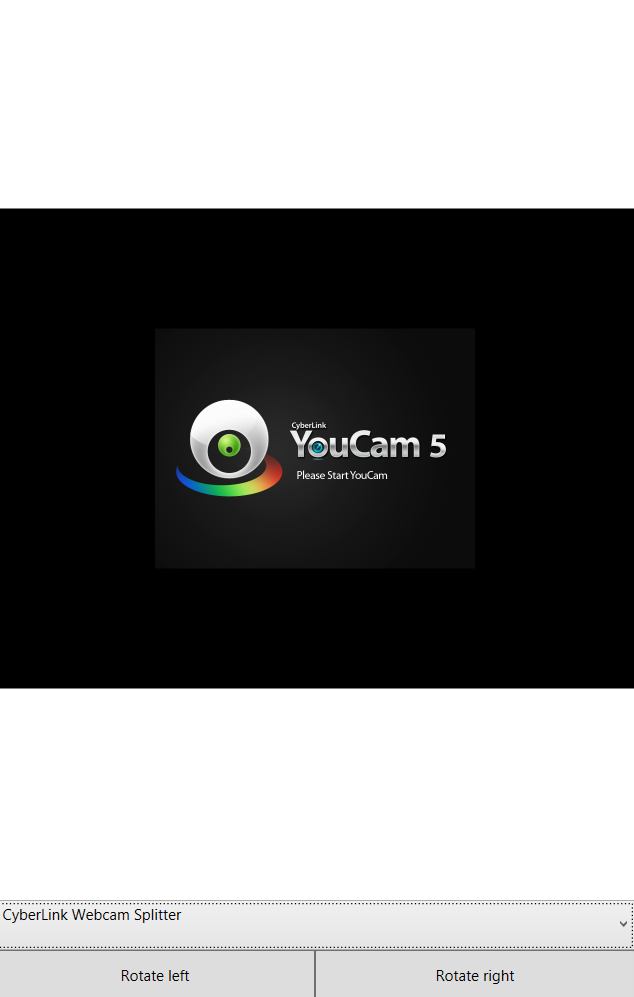
\includegraphics[scale=0.5]{channelcontrol_screen}
\caption[Widok aplikacji]{Kontrolki \textit{ChannelControl}.}
\end{figure}

Aplikacja w trakcie działania, za pomoca oddzielnego wątku wywołuje metodę \textit{UpdateFrames} w serwisie {IViewProviderService}, która wywołuje pobranie obrazu z kamery. Następnie za pomocą metody \textit{GetCurrentViewAsBitmaps} z tego samego serwisu otrzymuje obrazy z obu kamer w formacie \textit{System.Drawing.Bitmap} i ładuje je do kontrolek wyświetlających obrazy, odświeżając widok całej aplikacji. \\
Zmiana źródła obrazu (kamery) możliwa jest poprzez wybór odpowiedniej opcji z listy ze wszystkimi dostępnymi źródłami. Wtedy za pomocą metody \textit{SetCapture} z serwisu ustawiamy wybrane źródło dla lewego lub prawego oka. \\
Obrót obrazu dokonywany jest za pomocą dwóch przycisków. Po kliknięciu jednego z nich następuje wywołanie metody \textit{RotateImage} z serwisu, która realizuje obrót o $90^\circ$ we wskazaną stronę dla odpowiedniego oka.

\pagebreak
\item [Kontrola przetwarzania obrazu] \hfill \\
Sterowanie przetwarzaniem obrazu możliwe jest tylko dla obu źródeł obrazu jednocześnie. Dlatego w głównym widoku umieszczona została jedna kontrolka \textit{SettingsControl}. Zawiera ona listę w postaci kontrolki \textit{System.Windonws.Control.ListBox} na której umieszczone zostały wszystkie dostępne w systemie obiekty do przetwarzania obrazu. W celu zarządzania tymi obiektami został stworzony szablon wyświetalny dla każdej pozycji z listy składający się z następujących elementów:

\begin{itemize}
\item Nazwa przekształcenia realizowanego przez obiekt.
\item Pole wyboru do aktywowania lub dezaktywowania wybranego przekształcenia.
\item Przycisk do przesunięcia na wcześniejsze miejsce na liście.
\item Przycisk do przesunięcia na kolejne miejsce na liście.
\end{itemize}

\begin{figure}[h]
\centering
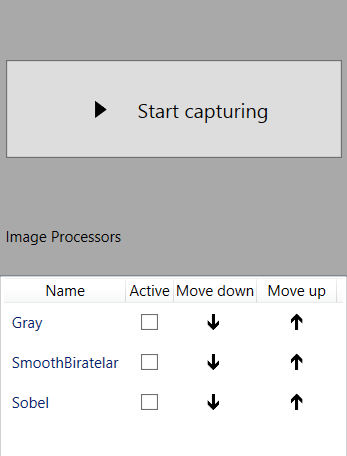
\includegraphics[scale=0.5]{settingscontrol_screen}
\caption[Widok aplikacji]{Kontrolka \textit{SettingsControl}.}
\end{figure}

Lista dostępnych przekształceń obrazu wraz z informacją o ich aktywności otrzymywana jest po wywołaniu metody \textit{GetAllImageProcessors} z serwisu \textit{IViewProviderService}. \\
Za pomocą dwóch stanów (zaznaczenie lub brak zaznaczenia) kontrolki \textit{System.Windows.Control.CheckBox} możliwe jest włączanie lub wyłączanie pojedynczych przekształceń. Po zmianie stanu kontrolki wywoływana jest metoda \textit{SetProcessorState}, która ustawia aktywność wybranego obiekty na wskazany stan. \\
Prezentowana lista odpowiada kolejnością liście obiektów przekształcających obraz.  Przekształcenia wykonywane są zaczynając od tego znajdującego się na górze listy. Zarządzanie tą kolejnością możliwe jest za pomocą przycisków, które przesuwają obiekt w dół lub w górę listy wywołując metodę serwisu o nazwie \textit{ChangeProcessorPriority}.

\end{description}

\subsection{Serwis komunikacji międzyprocesowej}

Ta część systemu odpowiada za komunikację pomiędzy procesem aplikacji Unity oraz procesem aplikacji konfiguracyjnej.  Do tego celu została wykorzystana technologia \textit{WCF}  (Windows Communication Foundation) stworzona przez firmę Microsoft. W założeniu, pierwszą uruchomioną aplikacją powinna być aplikacja Unity, która w momencie startu wystawia serwis w sieci lokalnej pod adresem \textit{http://localhost:{port}/OculusAR} gdzie port jest wartością pochodzącą z pliku konfiguracyjnego aplikacji. Aplikacja konfiguracyjna podczas uruchomienia próbuje się podłączyć do serwisu znajdującego się pod tym adresem, jeśli wystąpi błąd z połączeniem, użytkownik dostaje stosowny komunikat informujący o przyczynie błędu. 

Technologia \textit{WCF} wymaga, aby zdefiniować metody będące kontraktem dostępnych operacji, przez klasę, która obsługuje dany serwis. Kontrakt ten zdefiniowany został następująco:
\begin{figure}[h]
\centering
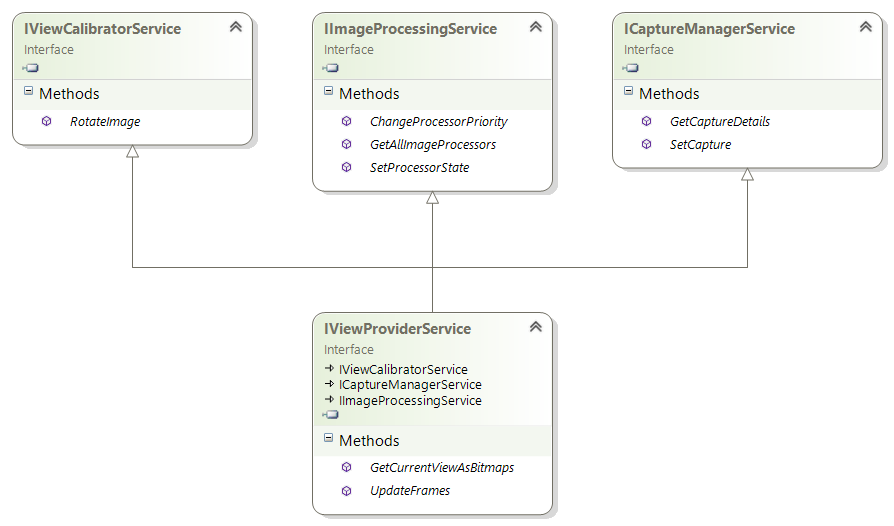
\includegraphics[scale=0.9]{IViewProviderService}
\caption[Serwisy diagram]{Interfejsy serwisów}
\end{figure}
 
Opis interfejsów zawartych w kontrakcie:
\begin{itemize}
\item \textit{IViewCalibratorService} - część serwisu odpowiadająca za rotację obrazu.
\item \textit{ICaptureManagerService} - część serwisu odpowiadająca za wybór źródła obrazu dla poszczególnych kanałów.
\item \textit{IImageProcessingService} - część serwisu odpowiadająca za zarządzanie przetwarzaniem obrazu.
tem \textit{IViewProviderService} - serwis składający się ze wcześniej wymienionych części oraz metod związanych z pobieraniem obrazu.
\end{itemize}

Szczegółowy opis metod zawartych w wymienionych interfejsach może zostać pominięty, ponieważ polegają one na wywołaniu metod o tych samych nazwach z klas implementujących interfejs \textit{IViewProvider}, którego opis znajduje się w poprzedniej części dokumentu.

Interfejs \textit{IViewProviderService} impelmentowany jest przez następujące klasy:

\begin{itemize}
\item \textit{ViewProviderService}
\item \textit{ViewProviderClient}
\end{itemize}

Pierwsza z nich odpowiada za utworzenie serwisu pod wspomnianym wcześniej adresem i wykorzystywana jest przez aplikację Unity, która tworzy serwis w momencie startu.
Natomiast druga klasa jest klientem, który podłącza się do istniejącego serwisu. Metody klienta polegają na wywołaniu metod serwisu o tej samej nazwie. Klasa ta wykorzystywana jest w aplikacji konfiguracyjnej , która za jej pomocą  może sterować procesem pobierania i przetwarzania obrazu w procesie aplikacji Unity.

 

\chapter{Rezultat pracy}
Ten rozdział jest poświęcony przedstawieniu rezultatów pracy nad omawianym systemem. Omówione zostaną testy, które zostały przeprowadzone w celu zbadania, czy stworzone rozwiązanie odpowiada założeniom, przedstawionym w rozdziale \textit{Cel i założenia projektu}. Rozdział obejmuje także omówienie wniosków wyciągniętych podczas pracy nad tworzonym systemem. 

\section{Konstrukcja gogli}
W celu zapewnienia wrażenia rozszerzonej rzeczywistości niezbędne było zamontowanie kamer na goglach wirtualnej rzeczywistości. Dzięki odpowiedniemu montażowi, uwzględniającemu cechy ludzkiej wizji stereoskopowej uzyskuje się gogle, które wyświetlają użytkownikowi obraz stereoskopowy oraz reagują na ruch głowy, poprzez ruch kamer.
Sposób montażu musiał spełniać dwa wymagania:
\begin{enumerate}
\item Niedozwolone są jakiekolwiek stałe modyfikacje gogli.
\item Montaż musi umożliwiać łatwą zmianę odległości między kamerami.
\end{enumerate}
W związku z tymi wymaganiami, wykorzystano już zamontowany do gogli uchwyt kontrolera Leap Motion. Kamery zostały przymocowane do uchwytu, składającego się z trzech części:
\begin{enumerate}
\item Dwa komponenty, bezpośrednio przymocowane do kamer.
\item Prowadnica, kształtem odpowiadająca kontrolerowi Leap Motion, do której te komponenty zostały przymocowane.
\end{enumerate}

-- projekt uchwytu

Uchwyt umożliwia przesuwanie kamer po prowadnicy w celu regulacji odległości między kamerami.

Projekt uchwytu wykonał <imię nazwisko> - członek Koła Naukowego Wirtualnej Rzeczywistości, absolwent wydziału MiNI. -- nie jestem pewien, czy to umieszczać w pracy, ale jednak warto o nim wspomnieć bo on to zaprojektował, do konsultacji.

-- zdjęcie gogli z zamontowanymi kamerami

\section{Testy rozwiązania}
Przeprowadzone testy można podzielić na dwie kategorie. Pierwszą z nich będą testy obiektywne, czyli takie, które można przedstawić w formie danych liczbowych. Tego typu testy będą związane bezpośrednio z wydajnością systemu i jej wpływem na wrażenia użytkownika. Drugą kategorią będą testy subiektywne, opierające się na indywidualnych odczuciach związanych z korzystaniem z kostruowanych gogli AR. 

\subsection{Testy wydajności}
Ten podrozdział jest poświęcony testom wydajności systemu. W związku z tym, że tego typu systemy należą do klasy tzw. systemów czasu rzeczywistego, jest to bardzo istotna kwestia przy tworzeniu takich rozwiązań. Nawet minimalne przekroczenie akceptowalnych przez ludzki organizm opóźnień może bardzo wpłynąć na komfort i ogólne wrażenie z korzystania z gogli.

\begin{description}
\item[Opóźnienie przesyłanego obrazu] \hfill \\
Pierwszą z kwestii, która została poruszona jest opóźnienie przesyłania obrazu na linii kamery - gogle. Jest to prawdopodobnie najważniejszy problem, od rozwiązania którego zależy to, czy system będzie nadawał się do użytku. Zbyt duże opóźnienia spowodują, że użytkownik nie będzie w stanie zareagować w odpowiednim czasie na zmiany w otoczeniu, ponieważ informacja o nich dotrze do niego za późno. W ramach testów zmierzono różnicę między czasem wyświetlanej klatki, a czasem rzeczywistym.

\textit{Sposób wykonania testu}

Założenia:
\begin{enumerate}
\item Różnicę czasu między wyświetleniem obrazu w aplikacji Unity, a w goglach VR przyjmujemy jako 0 ms. Nie mamy wpływu na zmianę tego opóźnienia bez ingerencji w kod biblioteki zewnętrznej, zatem nie obejmujemy testami tego opóźnienia.
\item Pomiary wykonywane są przy dwóch podłączonych kamerach. Obie pobierają obraz z taką samą rozdzielczością.
\end{enumerate}

Do wykonania testu potrzebne są: kamera, ekran, stoper. Kamerę, która będzie wykorzystywana przez aplikację do pobierania obrazu, kierujemy w stronę ekranu. Stoper opieramy o ekran tak, aby był widziany przez kamerę. Jeżeli wszystko jest ustawione poprawnie, to na ekranie stoper powinien być widoczny dwukrotnie. Widziany bezpośrednio przez kamerę oraz wyświetlany na ekranie. Oba obrazy stopera powinny być na tyle czytelne, aby zatrzymując obraz można było odczytać z niego czas.
Różnica pomiędzy czasem, wyświetlanym na bezpośrednim obrazie stopera, a czasem z jego obrazu ekranowego, jest opóźnieniem danej klatki.
Należy wykonać kilka pomiarów, a następnie na ich podstawie wyznaczyć opóźnienie obrazu (i niepewności pomiarowe?)

\textit{Wyniki}
TODO

\item[Ilość klatek na sekundę] \hfill \\
TODO - wstęp, wpływ na user-experience

\textit{Sposób wykonania testu}
TODO

\textit{Wyniki}
TODO

\end{description}


\subsection{Testy użytkowe}

W tym podrozdziale omówione zostaną testy, które zostały wykonane pod kątem zbadania ogólnego wrażenia użytkownika, który korzysta z konstruowanych gogli AR. Podczas testów uwaga była skierowana w stronę uzyskania jak najlepszego odwzorowania naturalnej wizji ludzkiej. W tym celu sprawdzono czy człowiek, patrząc przez gogle, jest w stanie radzić sobie z czynnościami, które wymagają korzystania ze zmysłu wzroku, a które w normalnych warunkach nie stanowią problemu. Wykonując te testy sprawdzono w jaki sposób wydajność systemu, omówiona w poprzednim podrozdziale, wpływa na koordynację wzrokowo-ruchową człowieka wykorzystującego stworzony system.

TODO - powpisywać pomysły testów
\begin{description}
\item[Czytanie książki] \hfill \\
TODO Opis
\item[Odbijanie piłeczki pingpongowej] \hfill \\
TODO Opis
\item[Gra w łapki] \hfill \\
TODO Opis
\item[Chwytanie poruszającego się przedmiotu] \hfill \\
TODO Opis
\item[Celowanie laserem w punkt (statyczny lub dynamiczny)] \hfill \\
TODO Opis
\end{description}

\section{Wnioski}
TODO 

\subsection{Co wyszło dobrze}
TODO

\subsection{Co nie wyszło dobrze}
TODO

\chapter{Przyszłość rozwiązania}
TODO

\section{Dalszy rozwój systemu}
TODO

\subsection{Usprawnienia}
TODO
\begin{enumerate}
\item Zwiększenie wydajności
\item Ograniczenie przewodów
\item Powiększenie pola widzenia
\end{enumerate}

\subsection{Dodatkowe funkcjonalności}
TODO
\begin{enumerate}
\item Wykrywanie ruchu gałki ocznej
\item Pobieranie informacji o ruchu głowy
\item Opracowanie szybkiego przesyłu obrazu na odległość
\end{enumerate}

\section{Potencjalne zastosowania}
TODO
\begin{enumerate}
\item Zdalnie sterowane roboty
\item Zdalnie pilotowane drony
\item Zdalne oglądanie np. mieszkań
\end{enumerate}

% -------------------- 6. Bibliografia -----------------------
% Bibliografia leksykograficznie wg nazwisk autorów

\begin{thebibliography}{20}%jak ktoś ma więcej książek, to niech wpisze większą liczbę
% \bibitem[numerek]{referencja} Autor, \emph{Tytuł}, Wydawnictwo, rok, strony
% cytowanie: \cite{referencja1, referencja 2,...}

\bibitem[1]{Ktos} A. Aaaaa, \emph{Tytuł}, Wydawnictwo, rok, strona-strona.
\bibitem[2]{Innyktos} J. Bobkowski, S. Dobkowski, \emph{Blebleble}, Magazyn nr, rok, strony.
\bibitem[3]{B} C. Brink, \emph{Power structures}, Algebra Universalis 30(2), 1993, 177-216.
\bibitem[4]{H} F. Burris, H. P. Sankappanavar, \emph{A Course of Universal Algebra}, Springer-Verlag, New York, 1981.
\end{thebibliography}
\thispagestyle{empty}


% --- 7. Wykaz symboli i skrótów - jeśli nie ma, zakomentować
\chapter*{Wykaz symboli i skrótów}

\begin{tabular}{cl}
nzw. & nadzwyczajny \\
* & operator gwiazdka \\
HUD & head-up display \\
FPS & frames per second \\
IDE & Integrated Development Environment \\
HTTP & Hypertext Transfer Protocol \\
$\widetilde{}$ & tylda
\end{tabular}
\thispagestyle{empty}


% ----- 8. Spis rysunków - jeśli nie ma, zakomentować --------
\listoffigures
\thispagestyle{empty}


% ------------ 9. Spis tabel - jak wyżej ------------------
\renewcommand{\listtablename}{Spis tabel}
\listoftables
\thispagestyle{empty}



% 10. Spis załączników - jak nie ma załączników, to zakomentować lub usunąć

\chapter*{Spis załączników}
\begin{enumerate}[itemsep = 0pt]
\item Załącznik 1
\item Załącznik 2
\end{enumerate}
\thispagestyle{empty}

% --------------------- 11. Załączniki ---------------------
% to jest po to, żeby było wiadomo, że załączniki znajdują się na końcu pracy

\newpage
\pagestyle{empty} 
Załącznik 1, załącznik 2
\end{document}
